\chapter{Understanding CUDA}\label{chp:GPGPU}

\chapterquote{Hardware: The parts of a computer system that can be kicked.}{Jeff
  Pesis}

% Motivate the use of GPUs

Because of the evergrowing demand for new visual effects and more detail in
computer games and other 3D graphics applications, GPUs have seen a massive
increase in computational power and potential memory bandwidth over the last
decade. This is evidenced by \reffig{fig:gpuCpuCompare}, which compares the
development of NVIDIA's GPUs with that of Intel's CPUs. These figures illustrate
the potential performance gain associated with implementing computationally
heavy solutions on todays GPUs instead of CPUs. The first figure,
\reffig{fig:gpuCpuGFLOPS}, compares the computational capacity and shows how the
theoretical number of floating point operations have increase over the last
decade, with GPUs being able to perform nearly 1500G floating point operations
per second as of the GeForce 480 GTX series, while Intel CPUs only reach around
200G operations. The second figure, \reffig{fig:gpuCpuThroughput}, compares the
memory bandwith of GPUs and CPUs. Memory bandwidth is the rate at which data can
be read from or stored into memory by one of the processing units and is around
6 times higher for the GPU than the CPU.

\begin{figure}
  \centering 

  \subfloat[Comparison of computational capacity in billions of floating point
    operations per second.]{ 
    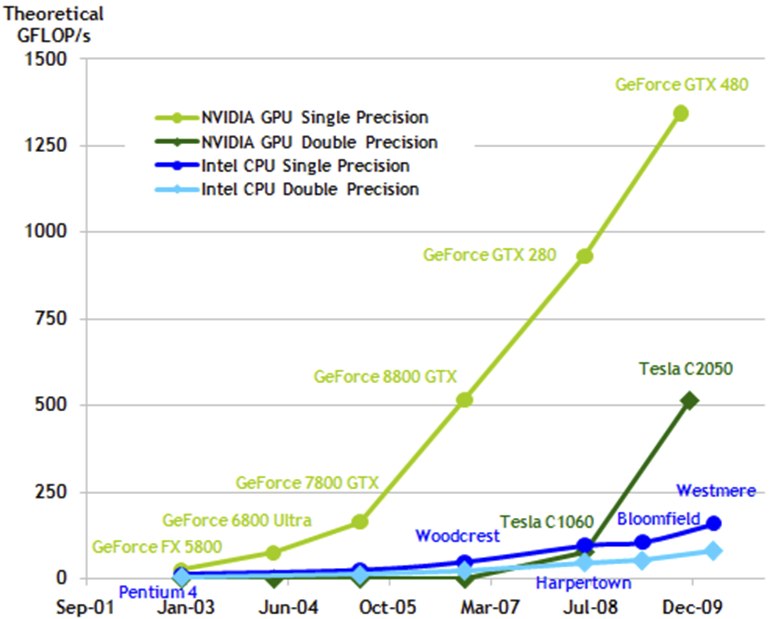
\includegraphics[width=0.45\textwidth]{GFLOPS}
    \label{fig:gpuCpuGFLOPS}
  }
  \hspace{0.05\textwidth}
  \subfloat[Comparison of memory bandwidth in gigabytes per second.]{
    \includegraphics[width=0.45\textwidth]{throughput}
    \label{fig:gpuCpuThroughput}
  }
  
  \caption[Comparison of FLOPS and memory bandwidth on GPUs and CPUs.]{A comparison
    of the development of floating point operations per second and memory
    bandwidth of GPUs and CPUs over the last decade. \\The figures are from chapter 1 in
    \citebook{CUDAPG}.}\label{fig:gpuCpuCompare}
\end{figure}

% What is different form CPUs

Utilizing the GPU's computational power and memory bandwidth effectively,
however, is not straightforward and in order to create algorithms for the GPU
that are executed faster than their CPU counterparts, we need an understanding
of how the GPU works.

The reason behind the difference in computational power and memory bandwidth
seen in \reffig{fig:gpuCpuCompare}, is that the CPU is designed for efficient
handling of control flow and with a large cache at its disposal. This enables it
to handle all kinds of applications, not just computationally intense ones. The
GPU on the other hand is designed for high throughput of small, arithmetically
intense, \textit{data parallel programs}\footnote{Each instruction is
  concurrently applied on multiple data elements.} called \textit{kernels},
which is exactly what is required of a graphics card that processes thousands of
independent vertices and performing the same color calculations, or
\textit{shading}, on hundreds of thousands of \textit{fragments}\footnote{A
  fragment contains all the data needed to generate the color of geometry in a
  single raster cell.}.

Since the graphics card is designed to perform vertex and fragment processing
independently of their respective neighbouring threads, this means that no
assumptions can be made about which thread is where in its execution when
programming the graphics card. This presents a problem in cases where the $n$'th
thread depends on information from all previous $n-1$ threads, e.g. when
shuffling elements in a list or calculating the minimum or maximum values of a
list of vertices. NVIDIA's CUDA framework remedies this somewhat by providing
synchronization primitives, but these can only synchronize a subset of the
running threads. The general problem of passing information between threads is
therefore not solved by CUDA's synchronization primitive alone.

% Why not use GPU/CPU solutions

An obvious solution is of course to perform easily parallelisable operations on
the graphics device and leave the rest for the CPU, or \textit{host}. However,
the following quote comes to mind:

\quotebook{ It is important to include the overhead of transferring data to and
  from the device in determining whether operations should be performed on the
  host or on the device.}{CUDABPG}

So once it has been decided to use the graphics card, data should not be
transfered back and forth between the CPU and GPU too often. The transfer
overhead would in many cases outweigh the performance increase gained by using
the GPU in the first place.

%% Fortunately Sengupta et al. has come up with a solution to the
%% scattering problem, which will be discussed further in
%% \refsection{sec:GPUprims}.


% Overview of the chapter

Finding effective GPGPU\footnote{General-Purpose computation on Graphics
  Processing Units.} solutions to the above mentioned problems is the motivation
for this chapter, which is structured as follows. First we shall look at how
threads and memory are organized in CUDA. Understanding this will be critical in
developing efficient GPGPU solutions. Then a section will present a scan
primitive for GPU computing. In this section I will show why this new primitive
is useful and present a case where the data in a list is shuffled by threads
running in parallel. Something that could not have been done effectively without
the scan primitive. In the chapters final section I will discuss a couple of
general CUDA optimization techniques, while applying them to a case study.

\section{The Architecture of CUDA}

Understanding the architecture of CUDA requires us to first understand the
relationship and layout of threads and the different kinds of memory available
to these threads.

CUDA's architecture is based on \textit{multiprocessors}. Unlike a single
threaded CPU, a multiprocessor is able to execute hundreds of threads
concurrently. Managing these threads is made easier by the multiprocessors'
\textit{SIMT}\footnote{Single-Instruction, Multiple-Thread} architecture, in
which a single instruction in a program is relayed to several threads in
parallel. A multiprocessor is equipped with fast, but limited local memory,
which can be used by threads currently executing on the multiprocessor. These
multiprocessors enable the graphics card to handle execution of more than a
million threads per kernel launched.


\subsection{The Thread Hierarchy}\label{sec:threadHierarchy}

% Grid, blocks, warps and threads. We will only deal with the one
% dimensional case.

% warps

At the lowest level, threads are scheduled and executed completely parallel in
small groups called \textit{warps}\footnote{The term originates from weaving,
  the first parallel thread technology.\citebook{CUDAPG}}, with a warp size of 32
threads on current generation hardware. A thread in a warp has its own
instruction counter and register state, and can therefore branch independently
of neighbouring threads. However, a warp can only execute one specific
instruction at a time. The following example should help clarify this.

\begin{algorithmic}
  \IF{threadID < 16}
    \ASSIGN{$x$}{$threadID$}
  \ELSE
    \ASSIGN{$x$}{$32 - threadID$}
  \ENDIF
\end{algorithmic}

% It is a wide SIMD/SIMT, Single-Instruction / Multiple-Thread,
% machine. This means branching hurts. Alot!

The first 16 threads in the warp will evaluate the condition to true and thus
perform the assignment $x \leftarrow threadID$, while the next 16 threads will
evaluate it to false and execute the alternate statement $x \leftarrow 32 -
threadID$. Since a warp can only perform one distinct instruction at a time, it
will have to first execute $x \leftarrow threadID$, leaving the last 16 threads
idle. It next executes the else branch, meaning the first 16 threads are now
left idling. While this example shows how branching can hurt performance, when
all threads in a warp do not take the same execution path, knowning that all
threads in a warp are always executed synchronized can also be very beneficial,
which I will discuss in \refsection{sec:loopUnrolling}.

% TODO explain any/all/ballot?

% blocks

Warps are organized into 3 dimensional \textit{blocks} and all threads in a
block are expected to reside on the same multiprocessor, which provides a limit
as to how many threads a block can contain. On current generation GPU's the
limit can be up to 1024 threads per block or multiprocessor. The size of blocks
is chosen before a kernel is launched and all blocks allocated for that kernel
will have the same size. Threads can lookup their \textit{thread index} inside a
block through the 3 dimensional \textit{threadIdx} CUDA built-in variable. Being
able to lookup a threads index is important for working with data. In the one
dimensional case the $n$'th thread will usually process the $n$'th data
element. Without the thread index this would not be possible. Executing blocks
on the same multiprocessor enables us to synchronize the threads inside that
block at specific points in the kernel. This enables threads inside blocks to
cooperate on solving problems and allows them to share data through the
multiprocessor's fast local memory without fearing race conditions

% grid

Blocks are themselves arranged into the uppermost part of the thread hierarchy,
a 2 dimensional \textit{grid}. The amount of data being processed usually
defines how large the grid will be. Just like a thread can access its index, it
can also lookup its \textit{block index} inside the grid through the built-in
variable \textit{blockIdx}. A two dimensional thread hierarchy can be seen on
\reffig{fig:threadLayout}. The kernels in this thesis will usually process the
data as one dimensional linear lists, where a threads global index can be
calculated as 

\begin{displaymath}
  index = blockDim.x * blockIdx.x + threadIdx.x
\end{displaymath}

\begin{figure}
  \centering

  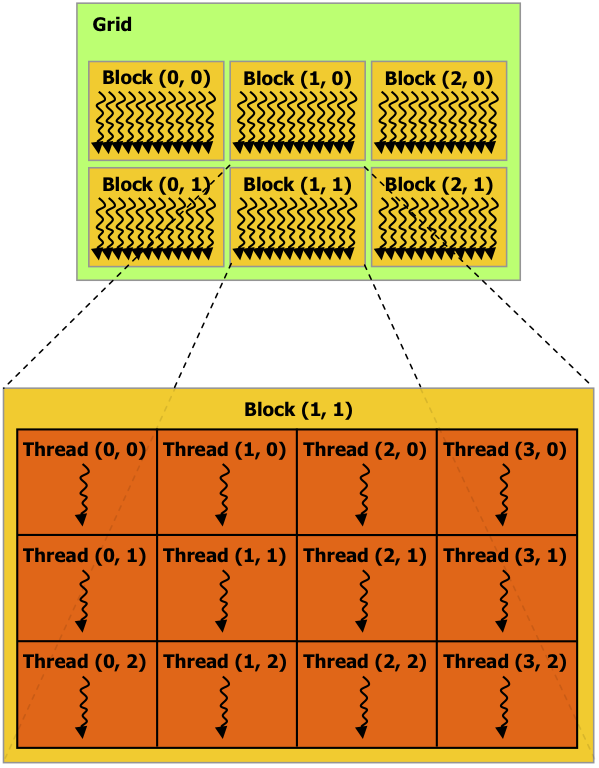
\includegraphics[width=8cm]{ThreadLayout}

  \caption[CUDA's thread hierarchy.]{A figure of CUDA's thread
    hierarchy.\\ The figure is from chapter 2 in \citebook{CUDAPG}.}
  \label{fig:threadLayout}
\end{figure}




\subsection{The Memory Model}\label{sec:memoryModel}

With the thread hierarchy explained, the different memory spaces made available
through CUDA can be described.

CUDA provides the programmer with three overall types of memory:

\begin{itemize}
\item \textit{global memory} - which can be accessed by any thread at any time
  and persists across kernel launches.
\item \textit{shared memory} - which is shared by all threads in a block and
  only persists for as long as that block is active.
\item \textit{registers} - which are local to each thread and only exists as
  long as its thread.
\end{itemize}

In the following I have devoted a subsection to each memory space.

\subsubsection{Global Memory}

% Slow, coalescene of data types with size 1, 2, 4, 8, and 16 bytes.

Global memory persists across kernel launches and is therefore perfect for
storing input data to kernels and their results. Unfortunatly it also has the
highest access time of the three memory spaces on CUDA devices. To avoid making
lots of memory transactions to and from global memory, a warp will try to
\textit{coalesce} its threads' global memory accesses into as few transactions
as possible. How well global memory access can be coalesced depends on the
\textit{compute capability} of the graphics hardware, with the coalescence
restrictions on newer GPUs being more flexible. Suffice it to say here that it
is preferable to access global memory sequentially, i.e. the $n$'th thread in a
warp accesses the $n$'th data element.

% Coalesced memory access, float4 instead of float3 The alignment requirement
% can be forced: stuct __align__(8) {

Another restriction on global memory is that data accessed must be of size 1, 2,
4, 8 or 16 bytes, otherwise memory transactions will be broken up into multiple
requests with an interleaved access pattern. Accesseing global data with an
interleaved access pattern hinders effective coalescence and should therefore
be avoided. Due to this, global memory access can be performed more efficiently
when using the CUDA built-in struct \textit{float4} instead of \textit{float3},
since \textit{float3} takes up 12 bytes and will be split into two memory
request with 8 and 4 bytes interleaved access patterns.

For more information on coalescence see Appendix G in \citebook{CUDAPG}, where
the coalescence requirements for hardware of a specific compute capability is
described.

% hiding latency

The scheduler will also help with hiding latency from global memory access. If
one warp is stalled while waiting for data, another warp that is resident on the
same multiprocessor and ready to execute can be scheduled instead. Utilization
of the graphics hardware is therefore heavily dependent on the number of
resident warps and maximizing these can be important. Especially in cases where
memory accesses are scattered, like they can become when the threads traverse
trees, such as the kd-tree. One way to increase the number of resident warps
will be introduced in the Registers and Local Memory section below.

% Mention textures and cache. The project developed for this thesis
% will not be using textures, since global memory also has cache as of
% 2.0 hardware.

\textit{Textures} also reside in device memory space. Textures are read only 1D,
2D or 3D data arrays that provide a fast texture cache optimized for 2
dimensional spatial data locality. This can make texture access faster than pure
global memory access, as a device memory read is only performed on a cache
miss. On current generation hardware however, global memory can use shared
memory as a cache, so textures will not be used in this project.

\subsubsection{Shared Memory}

% Faster than global/local. Allows threads to share data

Shared memory resides on the multiprocessor and is much faster than global
memory. It is shared by all threads in the same block and allows them to share
data.

% Used to overcome the limitations of global memory.

A normal usecase for shared memory is local caching of global data, which is
shared by multiple threads in the block. In this case the threads in a kernel
will cooperate on loading the data into shared memory, then the kernel will
perform a block-wide synchronization and proceed with operating on the data in
shared memory. When the kernel has finished its computations, the data can be
written back into global memory.

% Can be used as global cache on never CUDA architectures isntead of textures
% and shared mem. nice we laike

As mentioned above, on newer architectures multiprocessor memory can be used
implicitly as a cache for global memory.

% TODO? Bank conflicts, nothing is ever as good as it seems.



\subsubsection{Registers and Local Memory}

% Register

Registers are part of the threads execution context and is the fastest kind of
memory on the device. Since there is only a fixed amount of registers available
per multiprocessor, the register usage of a kernel's threads can have a high
impact on \textit{occupancy}\footnote{The number of warps resident on a
  multiprocessor, relative to the maximum amount possible.}, which in turn can
have an impack on the schedulers ability to hide memory latency.

% launch bounds

The compiler employs different heuristics to minimize register usage, while
ensuring that kernels run efficiently. Sometimes though, programmers may want to
use even fewer registers for specific kernels, in order to maximize occupancy
and global memory latency hiding. To this end they can aid the compilers
heuristics by providing \textit{launch bounds}. In CUDA two arguments can be
given as launch bounds. The first tells the compiler the maximum number of
threads per block that the kernel will ever be invoked with. The second argument
tells the compiler how many blocks should be resident on a multiprocessor. The
compiler can then use this information to derive upper bounds for the registers
available per thread.

% TODO? example



% Local memory

But the compiler cannot always simply reduce the number of registers to fit
inside the launch bounds. If a programmer specifies that a kernel's threads only
use 16 registers per thread, but each thread needs 20 registers to hold 20
distinct values, then those values have to be stored somewhere else. In that
case the compiler can use \textit{local memory}, which resides in device memory
and thus has the same high aceess latency as global memory. Forcing a few
registers into local memory to gain occupancy can be beneficial though, and
since all non-idling threads will access sequentially stored local memory at the
same time, there is a high probability that local memory access can be
coalesced.

Kernel variables that the compiler will most likely place in local
memory are:

\begin{itemize}
  \item Any array that from the compilers point of view is dynamically
    indexed.
  \item Structures or arrays that are to large to fit inside the
    registers.
  \item Any variable in the kernel if the kernel has to many variables
    to place them all in register memory. This is referered to as
    \textit{register spilling}.
\end{itemize}



\section{The Scan Primitive}\label{sec:GPUprims}

% Motivate

As explained above problems where the $n$’th thread requires information from
all previous $n-1$ threads can be quite hard to solve on data parallel
hardware. In this section I will outline a solution to the problem as presented
by \sengupta{} and give an example of how this solution can be used to sort a
list of data into two lists. In \refsection{sec:kdTreeImpl} we shall see that
being able to perform such sorting is important when associating triangles with
the children of a node that has been split.

% Prefix sum

An example taken from \sengupta{} showcasing this problem is the calculation of
a \textit{prefix-sum}, which is a special case of \textit{exclusive
  scan}. Exclusive scan takes as input a list of data, $[a_0, a_1, a_2, ...]$,
and a binary operator, $\oplus$, with an identity element, $i$. The result of
exclusive scan is then a new array with values $[i, a_0, a_0 \oplus a_1, a_0
  \oplus a_1 \oplus a_2, ...]$. For prefix-sum the operator is + and the
identity element is 0. An example of prefix-sum can be seen below:

\begin{displaymath}
  \begin{array}{r r r r r r r r r r}
    in: & 3 & 1 & 7 & 0 & 4 & 1 & 6 & 3 \\
    out: & 0 & 3 & 4 & 11 & 11 & 14 & 16 & 22 & 25 \\
  \end{array}
\end{displaymath}

Calculating the prefix-sum for $n$ elements on the CPU is trivial and can
naïvely be done with $O(n)$ memory accesses by iterating over the data array
from start to finish. A naïve implementation in the GPU however would require
each thread to sum up every previous value on its own, which would require
$O(n^2)$ memory accesses. Instead a data parallel algorithm has to be devised
that allows threads to cooperatively solve the problem and doing that as
efficiently as the CPU, i.e. with $O(n)$ memory accesses.


% Algorithm

As can be seen on \reffig{fig:segScan}, \sengupta{}'s work-efficient prefix-sum
requires two passes over the data, one called \textit{reduce} and another called
\textit{downsweep}. The object of the reduction phase is to calculate the sum of
all elements in the input list. It does so by applying the \textit{divide and
  conquer paradigm} and first solving the problem for subsections of the
list. Since only threads belonging to the same block can only be synchonized,
reduce only works on elements belonging to the same block. If the input list
holds more elements than can be reduced by a single block, then reduce is simple
applied to the result of the previous reduction until all values have been
reduced. The downsweep phase then makes use of the values computed by reduce to
produce the prefix-sum of the input list.

This is best described by the prefix-sum example on \reffig{fig:segScan}, where
the prefix-sum of a list of 8 elements is computed. I have chosen to reduce two
blocks to show how the first reduction result is combined into a new list and
then reduced further. Cells with the same color represent threads belonging to
the same block. The flow of data is represented as arrows, one arrow entering a
cell represents the data being copied, while two arrows entering a cell
represents an application of + on the two data elements and the result of that
application is then stored in the cell pointed to. After three steps each
individual block has reduced its own elements and the results are therefore
copied to an intermediate list for further reduction. When reduce is complete,
the downsweep phase begins. Downsweep first sets the last element in the current
list to the identity element, 0 in the case of prefix-sum, and then proceeds to
iteratively compute the prefix-sum. The result of applying the reduce and
downsweep is the prefix-sum of the input list, which can be seen in the final
list in \reffig{fig:segScan}.


%% The algorithm is depicted on \reffig{fig:segScan}. The figure shows scan
%% being applied to an array containing 8 elements. Cells with the same color
%% represent threads belonging to the same block. The arrows show how data is
%% moved, one arrow entering a cell represents a copy, while two arraws entering
%% represents the application of $\oplus$ to the data. The reduce phase in
%% \reffig{fig:segScan} shows how each block's threads are responsible for
%% cooperating on reducing their own values. If there are more data elements
%% than a single block can reduce on its own, then the reduce kernel is simply
%% applied repeatedly to the result of the previous reduce until the original
%% input has been reduced to a single element.

%% During down-sweep the data is pumped back out into the array and the values
%% calculated during the reduce phase are reused. The result of this is an array
%% containing the exclusive scan values. It can be quite instructive in data
%% parallel programming to go through this algorithm.


 
\newcommand{\drawArray}[4]{
  \draw (#1,#2) -> (#3,#2);
  \draw (#1,#4) -> (#3,#4);
  \foreach \x in {#1,...,#3} \draw (\x,#2) -> (\x,#4);
}

\begin{figure}
  \centering
  \begin{tikzpicture}[y=0.5cm, x=0.5cm,font=\sffamily]
    \draw (-0.8,0) -- (-1.2,0);
    \draw (-1,0) -- (-1,-5);
    \draw (-0.8,-5) -- (-1.2,-5);
    \node[rotate=-90] at (-1.5,-2.5) {Input List};

    \draw (-0.8,-6) -- (-1.2,-6);
    \draw (-1,-6) -- (-1,-13);
    \draw (-0.8,-13) -- (-1.2,-13);
    \node[rotate=-90] at (-1.5,-9.5) {Intermediate List};

    \draw (-0.8,-14) -- (-1.2,-14);
    \draw (-1,-14) -- (-1,-19);
    \draw (-0.8,-19) -- (-1.2,-19);
    \node[rotate=-90] at (-1.5,-16.5) {Input List};

    \node at (4, 1) {threads};
    \draw (0,0.5) -- (8, 0.5);
    \draw (0,0.3) -- (0,0.7);
    \draw (8,0.3) -- (8,0.7);

    \draw[-stealth] (10.5,-3) -- (10.5,-16);
    \node[rotate=-90] at (11,-9.5) {steps};
    
    \draw (8.8,0) -- (9.2,0);
    \draw (9,0) -- (9,-5);
    \draw (8.8,-5) -- (9.2,-5);
    \node[rotate=-90] at (9.5,-2.5) {1. reduce};

    % list
    \draw[line width=0.0pt, fill=lightgray] (8,0) -- (4,0) -- (4,-1) -- (8,-1);
    \drawArray{0}{0}{8}{-1}
    \draw (0.5,-0.5) node {3};
    \draw (1.5,-0.5) node {1};
    \draw (2.5,-0.5) node {7};
    \draw (3.5,-0.5) node {0};
    \draw (4.5,-0.5) node {4};
    \draw (5.5,-0.5) node {1};
    \draw (6.5,-0.5) node {6};
    \draw (7.5,-0.5) node {3};
    
    % Arrows
    \draw[applyOp] (0.5,-1) -> (1.5,-2);
    \draw[applyOp] (1.5,-1) -> (1.5,-2);
    \draw[applyOp] (2.5,-1) -> (3.5,-2);
    \draw[applyOp] (3.5,-1) -> (3.5,-2);
    \draw[applyOp] (4.5,-1) -> (5.5,-2);
    \draw[applyOp] (5.5,-1) -> (5.5,-2);
    \draw[applyOp] (6.5,-1) -> (7.5,-2);
    \draw[applyOp] (7.5,-1) -> (7.5,-2);

    % list
    \draw[line width=0.0pt, fill=lightgray] (8,-2) -- (4,-2) -- (4,-3) -- (8,-3);
    \drawArray{0}{-2}{8}{-3}
    \draw (0.5,-2.5) node {3};
    \draw (1.5,-2.5) node {4};
    \draw (2.5,-2.5) node {7};
    \draw (3.5,-2.5) node {7};
    \draw (4.5,-2.5) node {4};
    \draw (5.5,-2.5) node {5};
    \draw (6.5,-2.5) node {6};
    \draw (7.5,-2.5) node {9};

    % arrows
    \draw[applyOp] (1.5,-3) -> (3.5,-4);
    \draw[applyOp] (3.5,-3) -> (3.5,-4);
    \draw[applyOp] (5.5,-3) -> (7.5,-4);
    \draw[applyOp] (7.5,-3) -> (7.5,-4);
    
    % list
    \draw[line width=0.0pt, fill=lightgray] (8,-4) -- (4,-4) -- (4,-5) -- (8,-5);
    \drawArray{0}{-4}{8}{-5}
    \draw (0.5,-4.5) node {3};
    \draw (1.5,-4.5) node {4};
    \draw (2.5,-4.5) node {7};
    \draw (3.5,-4.5) node {11};
    \draw (4.5,-4.5) node {4};
    \draw (5.5,-4.5) node {5};
    \draw (6.5,-4.5) node {6};
    \draw (7.5,-4.5) node {14};

    % arrows
    \draw[applyOp] (3.5,-5) -> (0.5,-6);
    \draw[applyOp] (7.5,-5) -> (1.5,-6);

    \draw (2.8,-6) -- (3.2,-6);
    \draw (3,-6) -- (3,-9);
    \draw (2.8,-9) -- (3.2,-9);
    \node[rotate=-90] at (3.5,-7.5) {2. reduce};

    % list
    \drawArray{0}{-6}{2}{-7}
    \draw (0.5,-6.5) node {11};
    \draw (1.5,-6.5) node {14};
    
    % arrows
    \draw[applyOp] (0.5,-7) -> (1.5,-8);
    \draw[applyOp] (1.5,-7) -> (1.5,-8);

    % list
    \drawArray{0}{-8}{2}{-9}
    \draw (0.5,-8.5) node {11};
    \draw (1.5,-8.5) node {25};

    \draw (2.8,-10) -- (3.2,-10);
    \draw (3,-10) -- (3,-13);
    \draw (2.8,-13) -- (3.2,-13);
    \node[rotate=-90] at (3.5,-11.5) {1. d.s.};

    % list
    \drawArray{0}{-10}{2}{-11}
    \draw (0.5,-10.5) node {11};
    \draw (1.5,-10.5) node {0};

    % arrows
    \draw[applyOp] (0.5,-11) -> (1.5,-12);
    \draw[applyOp] (1.5,-11) -> (1.5,-12);
    \draw[applyOp] (1.5,-11) -> (0.5,-12);

    % list
    \drawArray{0}{-12}{2}{-13}
    \draw (0.5,-12.5) node {0};
    \draw (1.5,-12.5) node {11};

    % arrows
    \draw[applyOp] (0.5,-13) -> (3.5,-14);
    \draw[applyOp] (1.5,-13) -> (7.5,-14);

    \draw (8.8,-14) -- (9.2,-14);
    \draw (9,-14) -- (9,-19);
    \draw (8.8,-19) -- (9.2,-19);
    \node[rotate=-90] at (9.5,-16.5) {2. downsweep};

    % list
    \draw[line width=0.0pt, fill=lightgray] (8,-14) -- (4,-14) -- (4,-15) -- (8,-15);
    \drawArray{0}{-14}{8}{-15}
    \draw (0.5,-14.5) node {3};
    \draw (1.5,-14.5) node {4};
    \draw (2.5,-14.5) node {7};
    \draw (3.5,-14.5) node {0};
    \draw (4.5,-14.5) node {4};
    \draw (5.5,-14.5) node {5};
    \draw (6.5,-14.5) node {6};
    \draw (7.5,-14.5) node {11};

    % arrows
    \draw[applyOp] (1.5,-15) -> (3.5,-16);
    \draw[applyOp] (3.5,-15) -> (3.5,-16);
    \draw[applyOp] (3.5,-15) -> (1.5,-16);
    \draw[applyOp] (5.5,-15) -> (7.5,-16);
    \draw[applyOp] (7.5,-15) -> (7.5,-16);
    \draw[applyOp] (7.5,-15) -> (5.5,-16);
    

    % list
    \draw[line width=0.0pt, fill=lightgray] (8,-16) -- (4,-16) -- (4,-17) -- (8,-17);
    \drawArray{0}{-16}{8}{-17}
    \draw (0.5,-16.5) node {3};
    \draw (1.5,-16.5) node {0};
    \draw (2.5,-16.5) node {7};
    \draw (3.5,-16.5) node {4};
    \draw (4.5,-16.5) node {4};
    \draw (5.5,-16.5) node {11};
    \draw (6.5,-16.5) node {6};
    \draw (7.5,-16.5) node {16};

    % arrows
    \draw[applyOp] (0.5,-17) -> (1.5,-18);
    \draw[applyOp] (1.5,-17) -> (1.5,-18);
    \draw[applyOp] (1.5,-17) -> (0.5,-18);
    \draw[applyOp] (2.5,-17) -> (3.5,-18);
    \draw[applyOp] (3.5,-17) -> (3.5,-18);
    \draw[applyOp] (3.5,-17) -> (2.5,-18);
    \draw[applyOp] (4.5,-17) -> (5.5,-18);
    \draw[applyOp] (5.5,-17) -> (5.5,-18);
    \draw[applyOp] (5.5,-17) -> (4.5,-18);
    \draw[applyOp] (6.5,-17) -> (7.5,-18);
    \draw[applyOp] (7.5,-17) -> (7.5,-18);
    \draw[applyOp] (7.5,-17) -> (6.5,-18);

    % list
    \draw[line width=0.0pt, fill=lightgray] (8,-18) -- (4,-18) -- (4,-19) -- (8,-19);
    \drawArray{0}{-18}{8}{-19}
    \draw (0.5,-18.5) node {0};
    \draw (1.5,-18.5) node {3};
    \draw (2.5,-18.5) node {4};
    \draw (3.5,-18.5) node {11};
    \draw (4.5,-18.5) node {11};
    \draw (5.5,-18.5) node {15};
    \draw (6.5,-18.5) node {15};
    \draw (7.5,-18.5) node {22};

  \end{tikzpicture}

  %% \centering
  %% 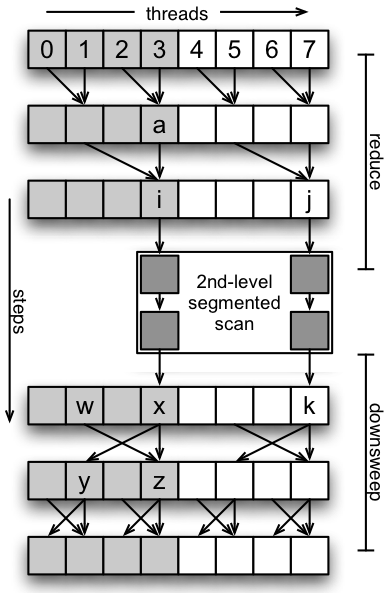
\includegraphics[width=4cm]{SegmentedScan}

  \parbox{8cm}{\caption[Segmented scan data flow.]{An example of segmented scan
      data flow. Cells with the same shading belong to the same block and the
      arrows represent data movement, either a copy or an application of
      $\oplus$.}\label{fig:segScan}}
\end{figure}

For specific details and further implementation optimizations see
\sengupta{}.


% time complexity

As can be seen on \reffig{fig:segScan}, the parallel scan performs $2 \cdot O(n
+ n/2 + n/4 + ... + 1) = O(n)$ memory accesses, since the memory accessed is cut
in half for each iteration of the reduce and down-sweep kernels.

% Useful for splitting data

Now the question is: \textit{why is this useful?}. The answer is that the
prefix-sum is vital to shuffling elements in lists on the GPU. Imagine a list of
triangles that have been split by a splitting plane and must now be sorted into
a new array. All the triangles in front of the plane will be sorted to the left
and the triangles behind it sorted to the right.

\begin{displaymath}
  \begin{array} {r r r r r r r}
    triangles: & [t_0 & t_1 & t_2 & t_3 & t_4 & t_5]\\
    side: & [r & l & r & l & l & r]\\
  \end{array}
  \Rightarrow
  \begin{array} {r r r r r r r}
    &[t_1 & t_3 & t_4 & t_0 & t_2 & t_5]\\
    &[l & l & l & r & r & r]\\
  \end{array}
\end{displaymath}

This needs to be done every time a tree node is split into two child nodes, so
being able to do this efficiently on the GPU is imperative to creating kd-trees
efficiently.

Obviously the individual threads in a split kernel will have no idea which
address to move the triangle to, since that depends on every other
thread. E.g. $t_0$ must move its data to entry 3, which it can only do if it
knows that it holds the first $r$ and that there are three $l$'s. However, by
first computing the prefix-sum of the $side$ list, while adopting the convention
that $r = 0$ and $l = 1$, splitting the triangles become quite easy. Using the
example above the prefix-sum becomes

\begin{displaymath}
  \begin{array} {r r r r r r r r}
    side: & [0 & 1 & 0 & 1 & 1 & 0]\\
    prefix\text{-}sum: & [0 & 0 & 1 & 1 & 2 & 3 & 3]
  \end{array}
\end{displaymath}

where the last element in $prefix\text{-}sum$ represents the total number of
triangles moved left, denoted $nf$.

The observant reader will have noticed that the prefix-sum actually calculates
the addresses where the triangles on the left side should be moved to. All that
remains is then to calculate the addresses of the triangles moved right. This is
done using $right_i = i - prefix\text{-}sum_i + nf$.

\begin{displaymath}
  \begin{array} {r r r r r r r}
    right: & [3 & 4 & 4 & 5 & 5 & 5]
  \end{array}
\end{displaymath}

The address that a thread should move its triangle to is then simply $address_i
= side_i == l$ ? $prefix_i$ : $right_i$ and becomes


\begin{displaymath}
  \begin{array} {r r r r r r r}
    address: & [3 & 0 & 4 & 1 & 2 & 5]
  \end{array}
\end{displaymath}

which will divide the triangles into their respective sides, just like
we wanted.

Sometimes the splitting planes used to split the nodes of a kd-tree will
intersect with some of the triangles in the scene and the triangle needs to be
associated with both the left and right side. In \refsection{sec:upperNodes} I
will show how this specific sorting problem can be solved.


% TODO? the data keeps its relation to other elements, which is good
% for coalescence.



\section{Optimization Techniques: Reduction}\label{sec:reduce}

% Motivation: Reduction was important in the previous step and will be again for
% median splitting

In the previous section we saw that it is important to be able to perform
\textit{reductions} efficiently on the GPU. A reduction is the processing of a
list of data in some order while building a return value.

%% Calculating the prefix-sum however isn't the only part of the kd-tree creator
%% where reductions are needed. It is also useful for calculating the bounding
%% boxes of the kd-tree's nodes, used when performing median splits.

In this section I present a naïve reduction algorithm and incrementally apply
CUDA specific optimizations to it. At the end of the section I present a table
summarizing the decrease in execution time after each applied optimization. The
reduction example will process the data using the binary operator \textbf{min},
with identity element $\infty$, and return the smallest value from the input
list, but the algorithm presented can easily be generalized to any binary
operator and its identity element. The naïve algorithm is based on the reduction
algorithm presented above and will perform $O(n)$ memory accesses, which is the
best we can hope for. Instead of improving the time complexity, the following
optimizations will instead focus on making better use of the GPU by hiding
latency, using faster memory where available and reduce the number of
calculations made.

% Works on individual blocks, must be run twice if input is too large for one
% block to handle.

The reduction algorithm will reduce values for individual blocks. If the input
list is too large to be reduced by one block, then the algorithm can be run
recursively on its own output, until a single result is found.

The algorithm presented assumes that the length of the input list is a power of
two. If that is not the case then either the data could be preprocessed or the
kernel itself can pad the data with the binary operators identity element.

\subsection{Naïve implementation}

The naïve algorithm, presented in \refalg{alg:naiveReduct}, is a
straight forward implementation of the interleaved access pattern
shown in \reffig{fig:segScan}. The algorithm uses the modulo operator
to distinguish which threads are done and which should continue to
perform reductions. All intermittent values are written back into
global memory, to allow other threads to access the reduced values
when needed. When the block has finished the reduction, the result
is returned by the first thread.

\begin{algorithm}
  \caption{Naïve reduction}
  \label{alg:naiveReduct}
  \begin{algorithmic}
    \PROCEDURE{Reduce0}
              {$values$ : Number List; $id$ : Integer; $elements$ : Integer}
              {$result$ : Number}
              {\ASSIGN{$offset$}{$1$}
                \WHILE{$id + offset < elements$}
                  \IF{$id$ \MOD $(offset * 2) = 0$}
                  \ASSIGN{$values[id]$}{\MIN{$values[id]$}{$values[id + offset]$}}
                  \ENDIF
                  \ASSIGN{$offset$}{$offset * 2$}
                  \SYNC
                \ENDWHILE
                \IF{$id = 0$}
                  \ASSIGN{$result$}{$values[0]$}
                \ENDIF
              }
  \end{algorithmic}
\end{algorithm}

\subsection{Coalesced Memory Access}

Of course there are several inefficiencies to correct in
\refalg{alg:naiveReduct}. To start with we will focus on global memory access
and update it to allow the warp to perform coalesced memory access. Since we are
interested in a global reduction it will not matter in which order values are
compared. This allows the interleaved access pattern to be exchanged with a
sequential one, which then lets the warp perform coalesced memory access.

%% Also better warp utilization as most threads are active and we get
%% rid of the slow mod operator.

Two pleasent side effects to this change, which is shown in
\refalg{alg:coalescedReduct}, is that the slow modulo operator has disappeared.
Warp utilization has also increased dramatically, since the first $offset$
threads in a block perform the same computations per iterations.
\begin{algorithm}
  \caption{Coalesced reduction}
  \label{alg:coalescedReduct}
  \begin{algorithmic}
    \PROCEDURE{Reduce1}
              {$values$ : Number List; $id$ : Integer; $elements$ : Integer}
              {$result$ : Number}
              {\ASSIGN{$offset$}{$elements / 2$}
                \WHILE{$offset > 0$}
                  \IF{$id < offset$}
                  \ASSIGN{$values[id]$}{\MIN{$values[id]$}{$values[id + offset]$}}
                  \ENDIF
                  \ASSIGN{$offset$}{$offset / 2$}
                  \SYNC
                \ENDWHILE
                \IF{$id = 0$}
                  \ASSIGN{$result$}{$values[0]$}
                \ENDIF
              }
  \end{algorithmic}
\end{algorithm}

% TODO? Figure of sequential access


\subsection{Working from Shared Memory}\label{sec:usingSharedMem}

Even with global memory access coalesced into fewer memory transactions,
continuously accessing global memory is still quite slow. To remedy this the
implementation in \refalg{alg:sharedReduct} first copies the data into shared
memory before performing any reductions. As can be seen the threads are working
together to perform the copy. Instead of all threads having to copy the entire
data, each thread only fills the $id$'th cell in the shared list and leaves the
other cells to be filled by the other threads. The subsequent synchronization
ensures that all the data has been copied before proceding with the
reduction. Since the threads are still accessing data sequentially, this change
preserves the coalesced memory fetches.

\begin{algorithm}
  \caption{Shared memory reduction}
  \label{alg:sharedReduct}
  \begin{algorithmic}
    \PROCEDURE{Reduce2}
              {$values$ : Number List; $id$ : Integer; $elements$ : Integer}
              {$result$ : Number}
              {\DECLARE{$sValues$}{\textbf{shared} Number List}
                \ASSIGN{$sValues[id]$}{$values[id]$}
                \SYNC
                \ASSIGN{$offset$}{$elements / 2$}
                \WHILE{$offset > 0$}
                  \IF{$id < offset$}
                  \ASSIGN{$sValues[id]$}{\MIN{$sValues[id]$}{$sValues[id + offset]$}}
                  \ENDIF
                  \ASSIGN{$offset$}{$offset / 2$}
                  \SYNC
                \ENDWHILE
                \IF{$id = 0$}
                  \ASSIGN{$result$}{$sValues[0]$}
                \ENDIF
              }
  \end{algorithmic}
\end{algorithm}

\subsection{Using Registers}

Shared memory is quite fast, but registers are even faster. Examining the
statement

\begin{displaymath}
  sValues[id] \leftarrow \text{\MIN{$sValues[id]$}{$sValues[id + offset]$}}
\end{displaymath}

we can see that the $id$'th thread will always access the value stored in
$sValues[id]$ and is the only thread writting to that cell. This provides us
with the possibility to use a register to store this value in instead of shared
memory. We still need to store the reduced value in shared memory though, for
when another thread needs the value in its next iteration. The resulting changes
can be seen in \refalg{alg:registerReduct}.

\begin{algorithm}
  \caption{Register reduction}
  \label{alg:registerReduct}
  \begin{algorithmic}
    \PROCEDURE{Reduce3}
              {$values$ : Number List; $id$ : Integer; $elements$ : Integer}
              {$result$ : Number}
              {\DECLARE{$sValues$}{\textbf{shared} Number List}
                \ASSIGN{$rValue \leftarrow sValues[id]$}{$values[id]$}
                \SYNC
                \ASSIGN{$offset$}{$elements / 2$}
                \WHILE{$offset > 0$}
                  \IF{$id < offset$}
                  \ASSIGN{$rValue \leftarrow sValues[id]$}{\MIN{$rValue$}{$sValues[id + offset]$}}
                  \ENDIF
                  \ASSIGN{$offset$}{$offset / 2$}
                  \SYNC
                \ENDWHILE
                \IF{$id = 0$}
                  \ASSIGN{$result$}{$rValue$}
                \ENDIF
              }
  \end{algorithmic}
\end{algorithm}



\subsection{Loop unrolling}\label{sec:loopUnrolling}

% Unroll the loops: Only works if the number of reductions are known
% beforehand (or if we pad the input)

The final optimization that will be applied to the reduction algorithm is
\textit{loop unrolling}. As stated above one of the assumptions made is that the
kernel knows beforehand how many elements a block will need to reduce. We now
extend this assumption with the condition that all blocks reduce the same number
of elements. Again this can be accomplished quite easily by padding the input
values when copying them to shared memory.

There are several reason as to why loop unrolling can increase
performance. Firstly looping requires indirection and even though most of the
threads in our warps will loop the same amount of times, the warps still incur
an overhead by having to perform the indirection. Secondly unrolling removes the
overhead of updating the $offset$ variable, which is a quite significant portion
of the work performed by the kernel when the body inside the loop is this
small. Thirdly we can take advantage of the synchronized execution of threads in
the same warp and remove explicit synchronization invocations when offset
becomes less than the warp size.

% Then move the first up to where data is loaded into shared mem. And
% move the last reduction down where the final result is written.

After having unrolled the loop, it is now also possible to move thread
0's last reduction, \MIN{$rValue$}{$sValues[1]$}, down to where the
result is output. We are also able to inline he first reduction, where
the data is copied from global memory to shared memory, reducing the
shared memory requirements by half per
block. \Refalg{alg:unrollReduct} shows the inlining of the first and
final reduction. Unrolling the loop is quite straightforward, but
takes a lot of space and has therefore been omitted here.

% Left as an exercise to the reader :)

\begin{algorithm}
  \caption{Unrolling reduction loops}
  \label{alg:unrollReduct}
  \begin{algorithmic}
    \PROCEDURE{Reduce4}
              {$values$ : Number List; $id$ : Integer; $elements$ : Integer}
              {$result$ : Number}
              {\ASSIGN{$offset$}{$elements / 2$}
                \DECLARE{$sValues$}{\textbf{shared} Number List}
                \ASSIGN{$rValue \leftarrow sValues[id]$}{\MIN{$values[id]$}{$values[id + offset]$}}
                \SYNC
                \ASSIGN{$offset$}{$offset / 2$}
                \WHILE{$offset > 1$}
                  \IF{$id < offset$}
                  \ASSIGN{$rValue \leftarrow sValues[id]$}{\MIN{$rValue$}{$sValues[id + offset]$}}
                  \ENDIF
                  \ASSIGN{$offset$}{$offset / 2$}
                  \SYNC
                \ENDWHILE
                \IF{$id = 0$}
                  \ASSIGN{$result$}{\MIN{$rValue$}{$sValues[1]$}}
                \ENDIF
              }
  \end{algorithmic}
\end{algorithm}

\subsection{Optimization results}\label{sec:optimizationResults}

The reduction algorithms above have been tested as part of a kd-tree
construction on a scene consisting of 70k triangles. During kd-tree construction
the reduce kernels were executed 20 times and their total execution time can be
seen in \reffig{fig:optimizationResults} aswell as the decrease in execution
time for each optimized kernel relative to the performance of Reduce0. The final
Reduce4 algorithm decreased execution time by 85.2\% compared to the naïve
implementation. This shows us that knowledge of how the GPU works is essential
to creating efficient GPU implementations. In the rest of the thesis it can be
assumed that the above optimizations have been applied to kernels that could
benefit from them. In some cases the very nature of an algorithm makes it
impossible to apply certain optimizations, such as coalescing data fetches for
several threads traversing different parts of the kd-tree. In these cases I will
note the lack of optimization and may present other solutions that can be
applied instead.

\begin{figure}
  \centering
  \begin{tabular}{r | c | c |}
    \textit{Algorithm:} & 
    \begin{tabular}{c}\textit{Total} \\ \textit{execution time:}\end{tabular} &
    \begin{tabular}{c}\textit{Decrease in} \\ \textit{execution time:}\end{tabular} \\
    \hline\hline
    Reduce0: & 59822.1$\mu$s & 0.0\% \\
    \hline
    Reduce1: & 26515.1$\mu$s & 55.7\% \\
    \hline
    Reduce2: & 13410.3$\mu$s & 77.6\% \\
    \hline
    Reduce3: & 12474.4$\mu$s & 79.1\% \\
    \hline
    Reduce4: & 8839.62$\mu$s & 85.2\% \\
    \hline
  \end{tabular}
  
  \vspace{3mm}
  \parbox{9cm}{\caption[Result of CUDA optimizations.]{This table shows the
      total execution time of the different reduce kernels presented in
      \refsection{sec:reduce}. The final column shows the reduction in execution
      time compared with Reduce0.}\label{fig:optimizationResults}}
\end{figure}

